\section{Quartic: degree=4}
\label{sec.quartic}

\subsection{Objectives}
The assignment in this section is:
\begin{enumerate}
\item Complete the file \code{src/quartic.py} by writing a Python
  function which computes and returns the x-intercepts of a curve
  equation is \[y=a x^4 + b x^3 + c x^2 + d x + e\,.\]
\item You'll need to replace all occurances of \code{raise NotImplementedError()}
  with correct python code which passes the tests.
\item Test the function in GitHub Codespaces by running the file\\
  \code{test/test\_quartic.py}.
\end{enumerate}

\subsection{Overview}

We wish to find the roots of the quartic polynomial given by 
\[P(x) = ax^4 + b x^3 + c x^2 + d x + e\,.\]

We will do this by first finding
(approximating) a root, $r$, using a technique called \emph{binary
seach}.  We will determine which regions to search by examining the derivative

\[\frac{d}{dx} P(x) = 4ax^3 + 3b x^2 + 2c x + d\,.\]

Knowing root $r$, we know that $(x-r)$ is a factor of 
$a x^4 + b x^3 + c x^2 + d x + e$.  Once $(x-r)$ is factored out of $P(x)$
what remains is a cubic polynomial of the form $A x^3 + B x^2 + C x + D$.
We can find the roots of the cubic using the technique
explained in Section~\ref{sec.cubic}, thus obtaining the roots of
the quartic polynomial.


\subsection{The Math}


A polynomial of degree 4 has the form $P(x) = a x^4 + b x^3 + c x^2 +
d x + e$. If $a=0$ than $P(x)$ is really a cubic polynomial (degree 3)
and can be solved using the techniques described in
Section~\ref{sec.cubic}.

If $a<0$ then similar to what we did for the cubic polynomial in
Section~\ref{sec.cubic.math}, we instead find the roots of
$-P(x) = -a x^4 - b x^3 - c x^2 - d x - e$.  $P(x)$ and $-P(x)$ are guaranteed to
have the same roots, but the code in Python will be easier if we know
that $a >= 0$.


Two polynomial equations (for $P(x)$ and $\frac{d}{dx} P(x)$) are
plotted in Figure~\ref{fig.quartic}.

\begin{figure}
\centering
%% derived from https://tex.stackexchange.com/questions/357538/graph-of-a-parabola-on-pgfplots
%% Thanks to Stefan Pinnow
%%     https://tex.stackexchange.com/users/95441/stefan-pinnow

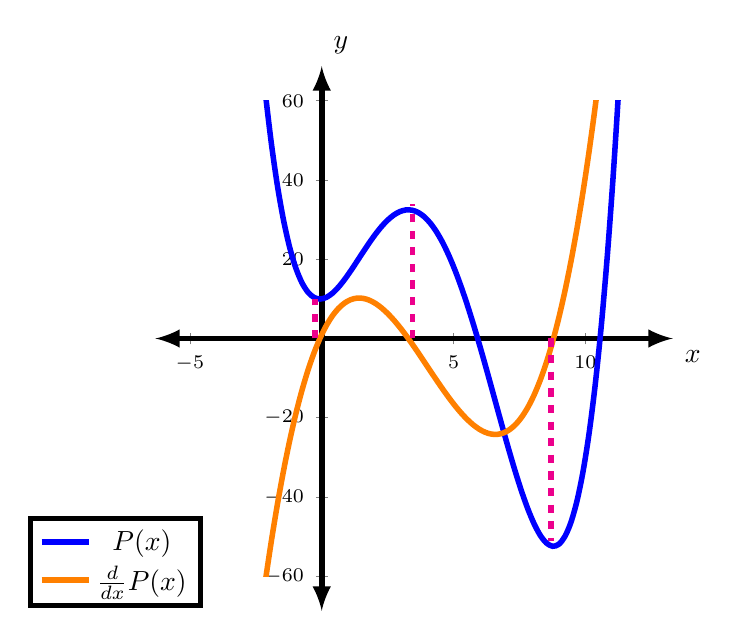
\begin{tikzpicture}
  \begin{axis}[
      samples=70,
      smooth,
      line width=2pt,
      domain=-4:12,
      legend pos=south west,
      legend style={
        anchor=east
      },
      width=0.6\textwidth,
      height=3in,
      axis lines=middle,
      xmin=-5,
      xmax=12,
      ymin=-60,
      ymax=60,
        scaled ticks=false,
        ticklabel style={font=\scriptsize},
        xlabel=$x$,
        ylabel=$y$,
        axis line style={
          latex-latex,
          shorten >=-12.5pt,
          shorten <=-12.5pt,
        },
        xlabel style={at={(ticklabel* cs:1)}, xshift=12.5pt, anchor=north west},
        ylabel style={at={(ticklabel* cs:1)}, yshift=12.5pt, anchor=south west},
    ]
    
    \addplot[color=blue] {0.125 * x^4 -2* x^3 + 7 * x^2 + x + 10};  
    \addlegendentry{\(P(x)\)}
    \addplot[color=orange] {0.5 * x^3 -6* x^2 + 14 * x + 1};
    \addlegendentry{\(\frac{d}{dx}P(x)\)}
    \draw[dashed,line width=1pt,line width=2pt,color=magenta] (3.45,0) -- (3.45,34);
    \draw[dashed,line width=1pt,line width=2pt,color=magenta] (8.7,0) -- (8.7,-51);
    \draw[dashed,line width=1pt,line width=2pt,color=magenta] (-0.25,0) -- (-0.25,10);
  \end{axis}
\end{tikzpicture}
%

\caption{Quartics}
\label{fig.quartic}
\end{figure}

\begin{align*}
  P(x) &= \frac{1}{8}  x^4 -2 x^3 + 7  x^2 + x + 6\\
  \frac{d}{dx} P(x) &= \frac{1}{2} * x^3 -6* x^2 + 14 * x + 1
\end{align*}

Notice that at the extreme left and right, the plot of $P(x)$ opens
upward, and the graph changes direction 3 times.  The values of $x$ at
which $P(x)$ changes direction are called the \emph{inflection
points}.  The inflection points are local minima of $P(x)$, and can
be computed by finding the values for which $\frac{d}{dx} P(x) = 0$.
Since the derivative of a degree 4 polynomial is a degree 3 (cubic)
polynomial, we can find where $\frac{d}{dx} P(x) = 0$ by using the
techniques explained in Section~\ref{sec.cubic}.

Once we have determined the 3 inflection points $x_1$, $x_2$, and $x_3$, we can
simply test $P(x_1)$, $P(x_2)$, $P(x_3)$.  If one if these values is 0, then
we have found a root, $r$, and we can factor $(x-r)$ out of $P(x)$ to obtain
a cubic polynomial.  We can find the roots of the cubic using the techniques
explained in Section~\ref{sec.cubic}.

If none of $P(x_1)$, $P(x_2)$, or $P(x_3)$ is zero, then we check
whether one of them is negative.  As shown in
Figure~\ref{fig.quartic}, whenever $P(x)<0$ then there is a root both
to the right and left of $x$.  If we can find that root, then as before
we can factor out $(x-r)$ to get a cubic polynomial, and then find its roots---
thus obtaining the roots of the quartic.

Once we have determined a root, $r$ of $P(x)$, then we know (similar
to the cubic case in Section~\ref{sec.cubic.math}) that $P(x)$ factors
into $(x-r)(Ax^3 + Bx^2 + Cx + D)$, where
\begin{align}
  A &= a\label{eq.7.A}\\
  B &= b + a r\nonumber\\
   &= b + A r\label{eq.7.B}\\
  C &= c + b r + a r^2\nonumber\\
  &= c + (b + a r)r\nonumber\\
  &= c + B r\label{eq.7.C}\\
  D &= d + c r + b r^2 + a r^3\nonumber\\
  &= d + ( c + b r + a r^2)r\nonumber\\
  &= d + C r\label{eq.7.D}
\end{align}

\subsection{The Programming}

Steps for finding the roots of a quartic polynomial.

\begin{enumerate}
\item Assume the coefficients of $P(x) = a x^4 + b x^3 + c x^2 + d x + e$ are
  \code{a},  \code{b},  \code{c},  \code{d}, and~\code{e}.
\item If \code{a==0}, then delegate to the previous solution by
  calling \\
  \code{find\_cubic\_roots} and returning its return
  value.  Be careful, \\
  \code{find\_cubic\_roots} accepts 4 input
  parameters.
\item Since $P(0) = e$, then we can easily evaluate the polynomial at
  $x=0$ to get its y-intercept.
  \begin{enumerate}
  \item If $e = 0$, then 0 is a root, $P(0) = 0$.
  \item If $e<0$ then there is a root on the positive x-axis and a
    root on the negative x-axis.  Find it with a binary search.
  \end{enumerate}
\item Find the inflection points by finding the roots
  of \[\frac{d}{dx} P(x) = 4 a x^3 + 3 b x^2 + 2 c x + d\,.\]
  \begin{enumerate}
  \item If $P(x)$ is zero at one of these inflection points, then the
    inflection point is a root.
  \item If $P(x) < 0$ at an inflection point, then there is a root
    both to the right and the left; find with by calling either
    \code{search\_root\_right} or \code{search\_root\_left}.
  \end{enumerate}
\item Once a root has been found, factor \[P(x) = (x-r)(Ax^3 + Bx^2 +
  Cx + D)\] by finding the coefficients, $A$, $B$, $C$, and $D$, using
  Equations~\eqref{eq.7.A} through~\eqref{eq.7.D}.
\item Find the roots of $Ax^3 + Bx^2 + Cx + D$ using
  \code{find\_cubic\_roots}.
  \item Concatenate the list of all the roots together to obtain the
    roots of the quartic polynomial.

\item Test your code by running the pre-defined tests in
  \code{tests/test\_quartic.py}.

\item Look at the proposed solution in \code{solutions/quartic.py}.
  It is not necessary that your code match exactly.

\end{enumerate}
